% Sources: original/9.4/*.png.
\chapter{Introduction to Ordinary Differential Equations}
\markboth{1. Introduction to Ordinary Differential Equations}{}

\begin{quote}
\centering\itshape
``An ODE is a law that tells us how a system changes.''
\end{quote}

An \textbf{ordinary differential equation} (ODE) relates an unknown
function of one variable to its derivatives.

\begin{exampleenv*}
Differentiation gives $y(t)=t^2\Rightarrow y'(t)=2t$; integration gives
$y'(t)=2t\Rightarrow y(t)=t^2+C$. Consider also $y'=y+2t$.
\end{exampleenv*}

\begin{exampleenv*}
For a falling object of mass $m>0$, with downward velocity $v=h'$,
\[
    mv'=mg,\qquad v'=g,\qquad h''=g.
\]
With linear air resistance, $mv'=mg-cv$ ($c>0$), and the equilibrium
velocity is $v=mg/c$.
\end{exampleenv*}

\begin{exampleenv*}
Unlimited population growth satisfies $P'=rP$, with solution
$P(t)=P_0e^{rt}$. With carrying capacity $K>0$, the logistic model is
\[
    P'=rP\left(1-\frac PK\right),\qquad r>0.
\]
\end{exampleenv*}

\Needspace{7\baselineskip}
\begin{exampleenv*}
A spring of stiffness $k>0$ attached to a mass $m>0$ satisfies
$mx''=-kx$. Its common solution and period are
\[
    x(t)=A\cos(\omega t)+B\sin(\omega t),\qquad
    \omega=\sqrt{\frac km},\qquad T=\frac{2\pi}{\omega}.
\]
\end{exampleenv*}

\begin{exampleenv*}
Newton's law of cooling is
\[
    T'=-k(T-T_a),\qquad k>0,
\]
where $T_a$ is the ambient temperature.
\end{exampleenv*}

\begin{remark*}
Initial conditions are specified independently of the ODE.
Analytic, qualitative, and numerical methods are used to study its solutions.
\end{remark*}

\section{Basic concept of ODE}

\begin{definitionenv}
An equation $F(x,y,y',\ldots,y^{(n)})=0$ is an \textbf{$n$-th order ODE}
if $y^{(n)}$ is the highest derivative involved.
It is \textbf{linear} if it can be written as
\[
    a_n(x)y^{(n)}+a_{n-1}(x)y^{(n-1)}+\cdots+a_1(x)y'+a_0(x)y=b(x);
\]
otherwise it is \textbf{nonlinear}.
\end{definitionenv}

\begin{exampleenv}
The equations $y'=xy$ and $y'=x^2$ are linear, whereas
\[
    y'=y^2,\qquad yy'=x,\qquad y''=y^2+x+\sin(y')
\]
are nonlinear. The equation $y'(x)=y(y(x))$ is not an ODE in this sense.
\end{exampleenv}

\begin{exampleenv}
For $y''+g=0$, the common solution is
\[
    y(t;c_1,c_2)=c_1+c_2t-\frac g2t^2.
\]
Additional conditions are needed to determine $c_1,c_2$.
\end{exampleenv}

\begin{remark}
Roughly speaking, a solution family of an $n$-th order ODE has $n$ free constants.
\end{remark}

\begin{definitionenv}
A \textbf{special solution} contains no free constants.
A family $y=\phi(x;c_1,\ldots,c_n)$ is a \textbf{common solution} of
$F(x,y,y',\ldots,y^{(n)})=0$ on an interval $J$ if
\[
    F\bigl(x,\phi,\partial_x\phi,\ldots,\partial_x^n\phi\bigr)=0
    \qquad(x\in J)
\]
for every parameter choice, and
\[
    \det\frac{\partial(\phi,\partial_x\phi,\ldots,\partial_x^{n-1}\phi)}
                  {\partial(c_1,\ldots,c_n)}\ne0.
\]
\end{definitionenv}

\begin{definitionenv}
If $\phi$ solves $y'=f(x,y)$ on $J$, its graph
\[
    \Gamma=\{(x,\phi(x)):x\in J\}
\]
is an \textbf{integral curve}. The \textbf{slope field} assigns the slope
$f(x,y)$ to each point $(x,y)$ in the domain of $f$.
\end{definitionenv}

\begin{theoremenv}
Let $\phi\in C^1(J)$. Its graph $\Gamma$ is an integral curve of
$y'=f(x,y)$ if and only if its tangent slope at each $(x,\phi(x))$ is
$f(x,\phi(x))$.
\end{theoremenv}

\begin{figure}[H]
    \centering
    \begin{minipage}{0.47\textwidth}
        \centering
        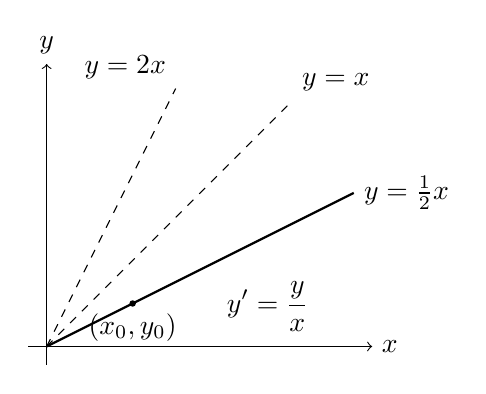
\begin{tikzpicture}[scale=0.78]
            \draw[->] (-0.3,0) -- (5.3,0) node[right] {$x$};
            \draw[->] (0,-0.3) -- (0,4.6) node[above] {$y$};
            \draw[dashed] (0,0) -- (2.1,4.2)
                node[above left] {$y=2x$};

            \draw[dashed] (0,0) -- (4.0,4.0)
                node[above right] {$y=x$};

            \draw[thick] (0,0) -- (5.0,2.5)
                node[right] {$y=\frac12x$};
            \fill (1.4,0.7) circle (1.5pt);
            \node[below] at (1.4,0.7) {$(x_0,y_0)$};
            \foreach \x in {2.0,2.7,3.4,4.1}
            {
                \draw
                ({\x-0.18},{0.5*\x-0.09})
                --
                ({\x+0.18},{0.5*\x+0.09});
            }
            \node[align=center] at (3.6,0.65)
            {$\displaystyle y'=\frac{y}{x}$};
        \end{tikzpicture}

        \[
            y=Cx
        \]
    \end{minipage}
    \hfill
    \begin{minipage}{0.47\textwidth}
        \centering
        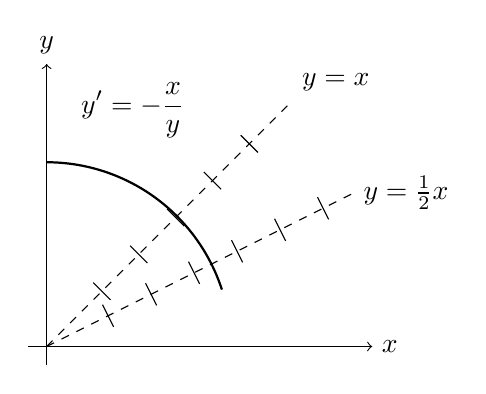
\begin{tikzpicture}[scale=0.78]
            \draw[->] (-0.3,0) -- (5.3,0) node[right] {$x$};
            \draw[->] (0,-0.3) -- (0,4.6) node[above] {$y$};
            \draw[dashed] (0,0) -- (4.0,4.0)
                node[above right] {$y=x$};

            \draw[dashed] (0,0) -- (5.0,2.5)
                node[right] {$y=\frac12x$};
            \foreach \t in {0.9,1.5,2.1,2.7,3.3}
            {
                \draw
                ({\t-0.14},{\t+0.14})
                --
                ({\t+0.14},{\t-0.14});
            }
            \foreach \t in {1.0,1.7,2.4,3.1,3.8,4.5}
            {
                \pgfmathsetmacro{\yy}{0.5*\t}
                \draw
                ({\t-0.09},{\yy+0.18})
                --
                ({\t+0.09},{\yy-0.18});
            }
            \draw[thick]
                plot[
                    domain=18:90,
                    samples=80,
                    variable=\a
                ]
                ({3.0*cos(\a)},{3.0*sin(\a)});

            \node at (1.4,3.85)
            {$\displaystyle y'=-\frac{x}{y}$};
        \end{tikzpicture}

        \[
            x^2+y^2=C
        \]
    \end{minipage}

    \caption{Integral curves and their slope fields.}
\end{figure}
